Per desenvolupar l'algorisme de control es parteix dels models elèctrics del
motor i de l'inversor. El tipus de motor a utilitzar defineix certes topologies
per l'inversor, que a la seva vegada determina les estratègies de control a
emprar. La possibilitat de disposar de sensors de posició i velocitat, la
robustesa que es vol assolir i el compromís entre complexitat i rendiment també
determinen les estratègies del control.

L'algorisme de control a implementar és de camp orientat (\emph{Field Oriented
Control}) amb una estratègia de control MTPA (\emph{Maximum Torque per
Ampere}). Amb objectiu de permetre unes velocitats superiors, es fa ús del
debilitament de camp (\emph{Field Weakening}). El control de camp orientat
requereix una tècnica de modulació per convertir el vector de voltatge a la
sortida del controlador en una tensió mesurada en les fases de l'inversor. Per
aquesta funció es fa servir el \acs{SVPWM}. El diagrama de la figura
\ref{simple} ens dóna una idea de com es relacionen aquests elements.

\begin{figure}[!htb]
    \centering
    \captionsetup{justification=centering, margin=1cm}
    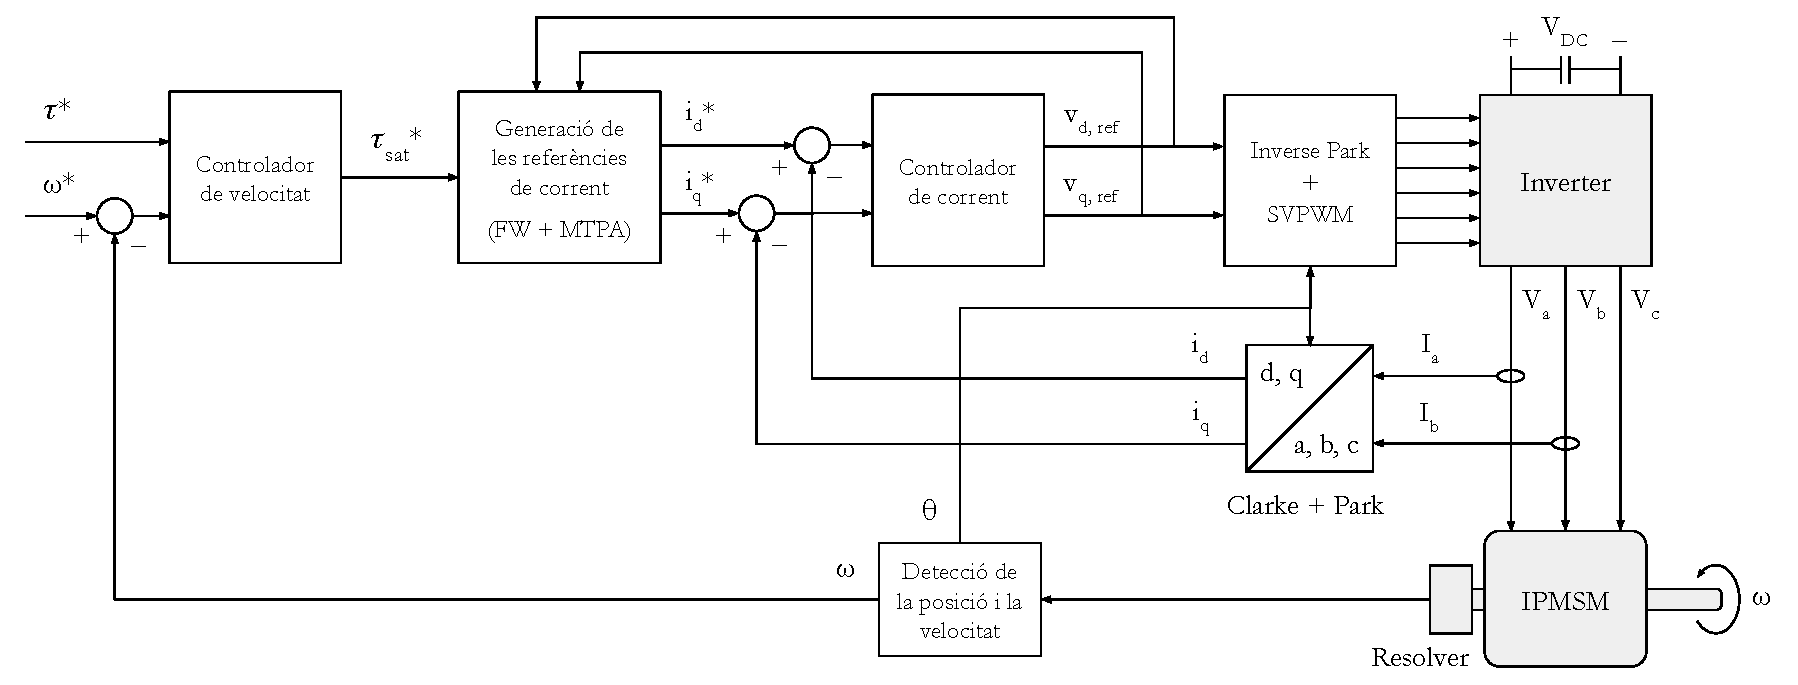
\includegraphics[width=14cm]
        { img/3_control_motor/simple.pdf }
    \caption[Diagrama de blocs del control]
        { Diagrama de blocs de l'algorisme control }
    \label{simple}
\end{figure}

\subsection{ Model elèctric del motor i de l'inversor }
{
    Un motor IPMSM es pot modelar a grans trets com una inductància i una
    resistència en serie per cada fase. En un motor trifàsic existeixen dos
    tipus de connexions, en estrella i en triangle. En el nostre cas, el
    connexionat és en estrella: les tres branques del motor s'uneixen en un
    punt intermig anomenat punt neutre i simbolitzat amb una $n$.

    L'equació de voltatges d'un motor síncron en el sistema de referència
    d-q\footnotemark per al nostre cas ve donada per l'equació 1:

    \footnotetext
    {   
        El sistema de referència d-q és un sistema de referència ortogonal
        bidimensional que es mou solidàriament amb el rotor. L'ús d'aquest
        sistema de referència linealitza alguns dels càlculs realitzats, que en
        cas contrari dependrien de la rotació del motor.
    }
    
    \begin{equation}
        \begin{bmatrix} v_d \\[5pt] v_q \end{bmatrix} =
        \begin{bmatrix}
            { R + \frac{d}{dt} L_d } & { -\omega L_q } \\[5pt]
            { \omega L_d } & { R + \frac{d}{dt} L_d }
        \end{bmatrix}
        \cdot \begin{bmatrix} i_q \\[5pt] i_d \end{bmatrix}
        + \begin{bmatrix} 0 \\[5pt] \omega \lambda_{pm} \end{bmatrix}
    \end{equation}

    on,
    \begin{description}
    {
        \item $\lambda_{pm}$ és el flux induït pels imats permanents al llarg de
        l'eix d-q
        \item $i_d, i_q$ són les components $d$ i $q$ del corrent induït
        \item $v_d, v_q$ són les components $d$ i $q$ del voltatge induït
        \item $L_d, L_q$ és la inductància del bobinat respecte als eixos $d$ i
        $q$
        \item $R$ és la resistència del bobinat
        \item $\omega$ és la velocitat angular del rotor
    }
    \end{description}

    \begin{figure}[!htb]
        \centering
        \captionsetup{justification=centering,margin=1.5cm}
        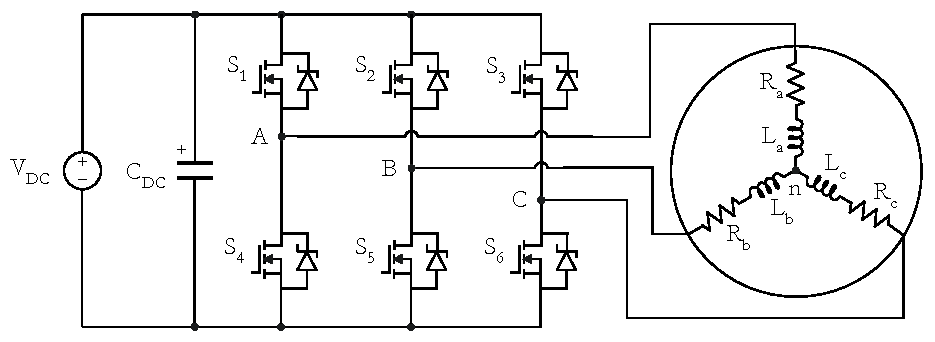
\includegraphics[width=12cm]
            { img/3_control_motor/inverter.pdf }
        \caption{ Circuit equivalent d'un inversor i motor trifàsics }
    \end{figure}

    Per conduir un motor trifàsic, l'inversor també ha de ser trifàsic. Cada
    una de les tres branques consta de dos transistors, formant el que
    es coneix com \emph{Half-Bridge}.
    
    La topologia emprada és la de dos nivells (\emph{Two Level Inverter, TLI}).
    L'elecció de la tipologia està justificada per membres anteriors de
    l'equip. A grans trets es pot dir que la decisió es basa en els següents
    factors:
    
    \begin{itemize}
        \item \textbf{Experiència:}
            L'equip disposa d'una experiència més amplia treballant amb
            inversors de dos nivells amb modulació per \ac{SVPWM}, ja que
            l'inversor Lenze actual presenta aquesta tipologia.

        \item \textbf{Bateria:}
            En cas d'implementar un inversor multinivell (MLI) la bateria
            hauria de dividir-se en dos, suposant un treball addicional per
            l'equip.

        \item \textbf{Estudi de pèrdues:}
            En l'estudi realitzat per l'equip, l'inversor TLI amb MOSFETs SiC i
            control per SVPWM va tenir les menors pèrdues per commutaci,
            aconseguint un aprofitament del bus DC del 90,7\% (no obstant, a
            costa d'una pitjor qualitat d'ona en termes de distorsió harmònica
            total, \acs{THD}).

        \item \textbf{Dimensions, pes i cost:}
            L'ús d'un inversor multinivell eleva el cost de l'inversor i el fa
            més voluminós i pesat en fer servir una major quantitat de
            transistors.

    \end{itemize}
}

\subsection{ Control de camp orientat }
{
    El control de camp orientat (\emph{Field Oriented Control}, FOC) és una de
    les tècniques de control més utilitzades quan es treballa amb motors
    d'imants permanents i motors d'inducció. Consisteix a controlar el corrent
    del motor una vegada sofert una sèrie de transformades (Park i Clarke) que
    sincronitzen els corrents amb el gir del rotor. En sincronitzar els
    corrents es poden aplicar tècniques de control lineal com els controladors
    proporcional-intregral (PI).

    \subsubsection{ Transformada de Clarke }
    {
        En un primer lloc, les mesures de corrent de les tres fases del motor
        (fases a, b i c) s'han de convertir a un sistema de referència de dos
        fases, formant l'espai estacionari $\alpha$-$\beta$. Per realitzar
        aquesta conversió s'empra la transformada de Clarke (o transformada
        $\alpha$-$\beta$ per la nomenclatura de les seves variables).
        L'expressió de la transformada de Clarke és la següent:

        \begin{equation}
            \begin{bmatrix} \alpha \\[5pt] \beta \\[5pt] \gamma \end{bmatrix} =
            \begin{bmatrix}
                \frac{2}{3} & -\frac{1}{3} & -\frac{1}{3} \\[5pt]
                0 & \frac{1}{\sqrt{3}} & -\frac{1}{\sqrt{3}} \\[5pt]
                \frac{1}{3} & \frac{1}{3} & \frac{1}{3}
            \end{bmatrix}
            \cdot \begin{bmatrix} a \\[5pt] b \\[5pt] c\end{bmatrix}
        \end{equation}

        La transformada de Clarke actua de manera que tots els punts situats
        sobre la semirrecta que surt de l'origen i creix paral·lela al vector
        de la fase $a$. De la mateixa manera, els punts situats sobre la
        semirrecta paral·lela a la fase $b$ passen a caure a sobre la
        semirrecta a 90º de la fase $a$.

        Com que el sistema trifàsic es de corrents balancejats, tenim que $i_a
        + i_b + i_c = 0$. Amb això, una de les tres branques de l'inversor
        (generalment el corrent anotat com $i_c$) es torna supèrflua, poguent
        simplificar així el càlcul de la transformada de Clarke. D'aquesta
        manera, l'equació implementada en el nostre cas pren la següent forma:

        \begin{equation}
            \begin{bmatrix} \alpha \\[5pt] \beta \end{bmatrix}
            = \frac{2}{3} \cdot
            \begin{bmatrix}
                1 & 0 \\[5pt]
                \frac{1}{\sqrt{3}} & \frac{1}{\sqrt{3}}
            \end{bmatrix}
            \cdot \begin{bmatrix} a \\[5pt] b \end{bmatrix}
        \end{equation}
    }

    \subsubsection{ Transformada de Park }
    {
        La següent transformació consisteix a cambiar el sistema de referència
        que té com vectors unitaris el vector paral·lel a l'eix del motor
        (conegut per vector directriu, annotat com $d$) i el vector perpendicular a
        aquest (conegut com vector de quadratura, annotat com $q$). En paraules
        llanes, es podria dir que ens muntem a sobre de l'eix del motor i
        començem a girar-hi solidàriament. És en aquest punt que la dependència
        amb l'angle desapareix i el valor de corrent resultant captura
        l'envolvent del senyal sinusoidal original. La transformació que
        s'empra per l'esmentat canvi és la transformada de Park, l'equació de
        la qual, en forma matricial, és:

        \begin{equation}
            \begin{bmatrix} q \\[5pt] d\\[5pt] 0 \end{bmatrix} = 
            \begin{bmatrix}
                cos(\theta) & sin(\theta) & 0 \\[5pt]
                -sin(\theta) & cos(\theta) & 0 \\[5pt]
                0 & 0 & 1
            \end{bmatrix}
            \cdot \begin{bmatrix} \alpha \\[5pt] \beta \\[5pt] \gamma \end{bmatrix}
        \end{equation}

        Veiem que per aplicar aquesta transformada necessitem el valor de
        l'angle del rotor. Aquest angle pot ser mesurat directament per mitjà
        d'un resolver o un encodificador, o d'altra banda es pot estimar a
        partir de les mesures de corrent fent servir observadors.
    }

    \subsubsection{ Transformada inversa de Park }
    {
        Un cop realitzat el control del corrent en el marc de referència d-q,
        la tensió obtinguda s'ha de transformar al marc de referència en el que
        opera el SVPWM, que es el d'$\alpha$-$\beta$. Per aquesta raó s'aplica
        la transformada inversa de Park, que s'obtè invertint la matriu de
        rotació de la transformada de Park:

        \begin{equation}
            \begin{bmatrix} \alpha \\[5pt] \beta \end{bmatrix} = 
            \begin{bmatrix}
                cos(\theta) & sin(\theta) \\[5pt]
                sin(\theta) & -cos(\theta) \\[5pt]
            \end{bmatrix}
            \cdot \begin{bmatrix} q \\[5pt] d \end{bmatrix} 
        \end{equation}
    }
}

\subsection{ Maximum Torque per Ampere }
{
    L'equació \ac{MTPA} ens permet obtenir el màxim parell donat un corrent
    determinat. L'equació es dedueix a partir del parell electromagnètic d'un
    motor PMSM, que pot ser expressat com:
    
    \begin{equation}
        \tau_{em} = \frac{3}{2}p(\lambda_{pm} i_q + (L_d - L_q) i_d i_q)
    \end{equation}

    on,
    \begin{description}
    {
        \item $\tau_{em}$ és el parell electromagnètic
        \item $\lambda_{pm}$ és el flux induït pels imats permanents al llarg
        de l'eix d-q
        \item $i_d, i_q$ són les components $d$ i $q$ del corrent induït
        \item $v_d, v_q$ són les components $d$ i $q$ del voltatge induït
        \item $L_d, L_q$ és la inductància del bobinat respecte als eixos $d$ i
        $q$
        \item $R$ és la resistència del bobinat
        \item $\omega$ és la velocitat angular del rotor
    }
    \end{description}

    Per obtenir un parell màxim, s'han de complir la següent condició
    d'optimització:
    
    \begin{equation}
        \left\{
            \begin{aligned}
                \frac{\partial (\tau_{em} / i_s)}{\partial i_d} = 0 \\
                \frac{\partial (\tau_{em} / i_s)}{\partial i_q} = 0
            \end{aligned}
        \right.
    \end{equation}

    Així, aplicant les condicions a l'equació de torque obtenim el corrent
    $i_d$ a injectar a partir del corrent $i_q$:

    \begin{equation}
        i_d = \frac{-\lambda_m + \sqrt{\lambda_m^2 + 4 (L_d - L_q)^2 i_q^2}}{ 2 (L_d - L_q) }
    \end{equation}

    % \begin{figure}[!htb]
    %     \centering
    %     \captionsetup{justification=centering, margin=1.5cm}
    %     \includegraphics[width=13cm]
    %         { img/3_control_motor/mtpa_fw.pdf }
    %     \caption[Regió de debilitament de camp]
    %         { Regió de debilitament de camp }
    %     \begin{quote}
    %         La regió en la que es produeix el debilitament de camp es troba
    %         limitada per les corves de \ac{MTPA} i \ac{MTPV}, així com les
    %         corves de corrent i voltatge màxims. 
    %     \end{quote}
    % \end{figure}
}

\subsection{ Debilitament de camp }
{
    El debilitament de camp o debilitament de flux (en anglés, \emph{Field
    Weakening}) és una tècnica per augmentar la velocitat d'un motor elèctric
    per damunt de la seva capacitat nominal, a càrreg de reduir el par motor.
    S'aplica en els casos en què es requereix obtenir una major velocitat i és
    admisible disposar de menor par motor. És molt utilitzada en motors
    d'imants pemanents, ja que es troben limitats en velocitat quan la tensió
    de l'estàtor assoleix el límit de sortida de l'inversor.

    El debilitament de camp fa ús dels corrents $i_q$i $q_d$ de l'inversor per
    contrarrestar el flux magnètic de l'entreferro que generen els imants del
    rotor. En específic, el control de debilitament de camp consisteix a reduir
    el flux de l'entreferro resultant associat als imants permanents,
    $\lambda_{pm}$, injectant un corrent $i_d$ negatiu.

    El debilitament de camp es pot implementar trobant la relació entre els
    corrents i la velocitat en aquest mode de funcionament, o bé tancant un
    llaç de control amb un controlador PI en el que la consigna sigui
    el valor de voltatge màxim del bus DC (multiplicat per un factor de
    seguretat) i la sortida el corrent $i_d$ necessari per mantenir el bus DC
    plenament utilitzat.
}

\subsection{ Modulació d'amplada de pulsos }
{ 
    Existeixen diverses tècniques de modulació d'amplada de pulsos. L'objectiu
    de la modulació d'amplada de pulsos és accionar els transistors de
    l'inversor per sintetitzar la tensió desitjada a cada una de les branques.

    Per a l'inversor de dos nivells les tècniques de modulació es reduixen a
    la pràctica a la modulació per mitjà de senyal sinusoidal o SPWM
    (\emph{Sinusoidal Pulse Width Modulation}) i a la modulació per mitjà de
    vectors espacials o SVPWM (\emph{Space Vectoring Pulse Width Modulation}).

    \subsubsection{ SPWM } 
    { 
        La modulació senoidal d'amplada de pulsos (\emph{Sinusoidal Pulse Width
        Modulation, SPWM}) és una tècnica de generació de PWM consistent a
        comparar el senyal de voltatge AC de referència amb un senyal portador
        triangular de freqüència igual a la freqüència de conmutació dels
        interruptors. Se sol utilitzar per la seva simplicitat a l'hora
        d'implementar-lo. Quan el senyal de referència es major que el senyal
        triangular, l'interruptor ``high" de la fase s'activa; en cas contrari,
        s'activa l'interruptor ``low".

        \begin{figure}[!htb]
            \centering
            \captionsetup{justification=centering, margin=1.5cm}
            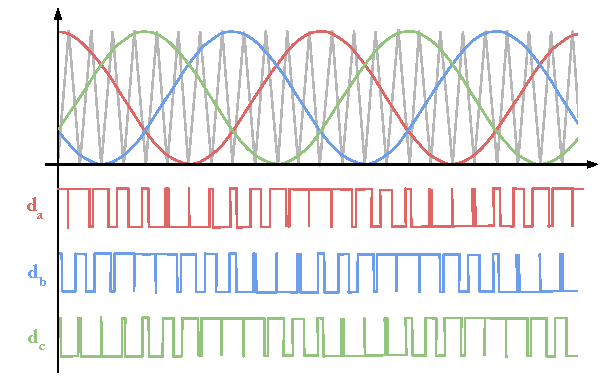
\includegraphics[width=7cm]
                { img/3_control_motor/spwm.pdf }
            \caption{ Generació dels cicles de treball en el SPWM.}
        \end{figure}
    }

    \begin{figure}[!htb]
        \centering
        \captionsetup{justification=centering,margin=1.5cm}
        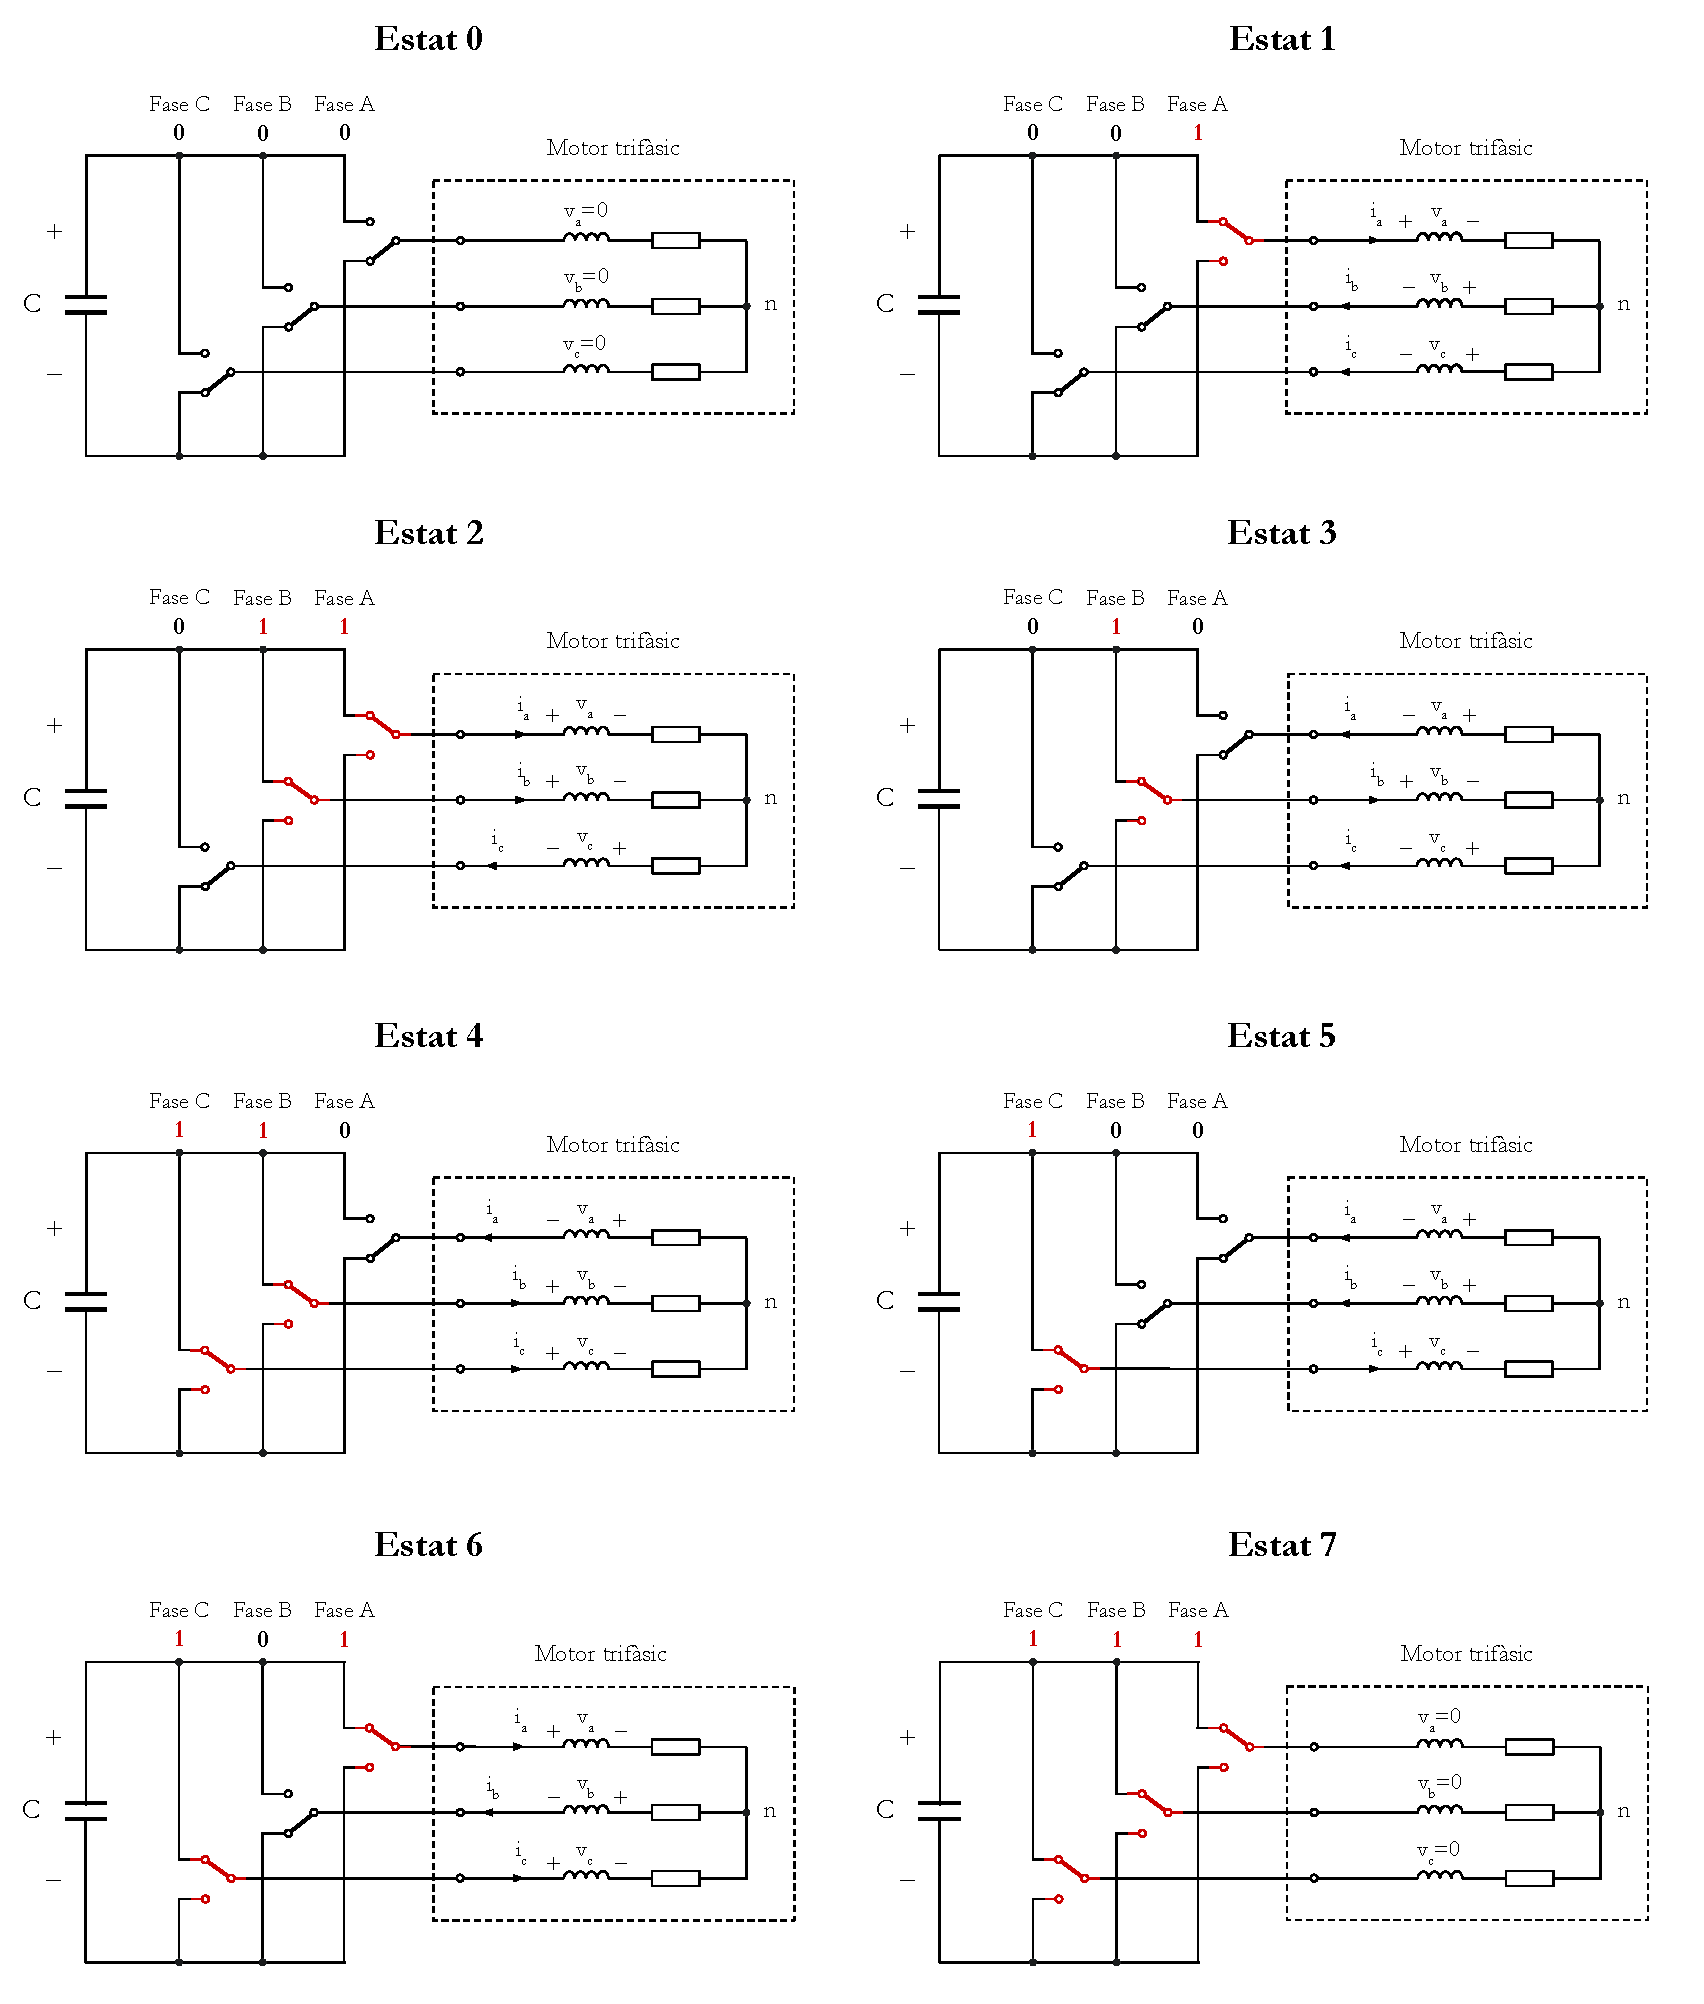
\includegraphics[width=14.5cm]
            { img/3_control_motor/states_inverter.pdf }
        \caption[Estats de l'inversor]
            { Estats de l'inversor}
        \label{estats}
    \end{figure}

    \newpage
    \subsubsection{ SVPWM } 
    { 
        La modulació d'amplada de pulsos per vectors espacials (SVPWM) empra la
        representació vectorial de un sistema polifàsic per generar el PWM. A
        gran trets l'objectiu es descomposar el vector de voltatge de
        referència en vectors associats a cada un dels estats de commutació
        d'un inversor. L'ús de la modulació SVPWM permet aprofitar el bus
        DC molt més que amb la modulació sinusoinal SPWM més tradicional, d'un
        90,7\% contra un 78,5\%.

        En un inversor trifàsic, cada branca compta amb un parell de
        transistors que treballen conjuntament com un commutador (i evitant el
        curtcircuit del bus DC). En tot moment els bobinats de cada branca del
        motor estan connectats al pol positiu o el negatiu del bus DC. Com que
        tenim a la nostra disposició 3 parells de transistors i dos estats
        posibles per branca, es configuren 8 estats, dos d'ells nuls (estats 0
        i 7), ja que no hi ha caiguda de tensió en cap dels bobinats del motor.
        La configuració dels possibles estats es pot veure en la figura
        \ref{estats}.

        Podem associar cada un d'aquests estats a un vector en l'espai de
        referència $\alpha\-\beta$, de manera que configuren un hexàgon,
        caracterísitc del SVPWM, tal i com es representa en la figura
        \ref{hexagon}. Així, es generen 6 sectors diferents delimitats pels
        vectors dels estats 1 a 6. Els estats 0 i 7, per la seva banda, queden
        en el centre del sistema de referència.

        \begin{figure}[!htb]
            \centering
            \captionsetup{justification=centering,margin=1.5cm}
            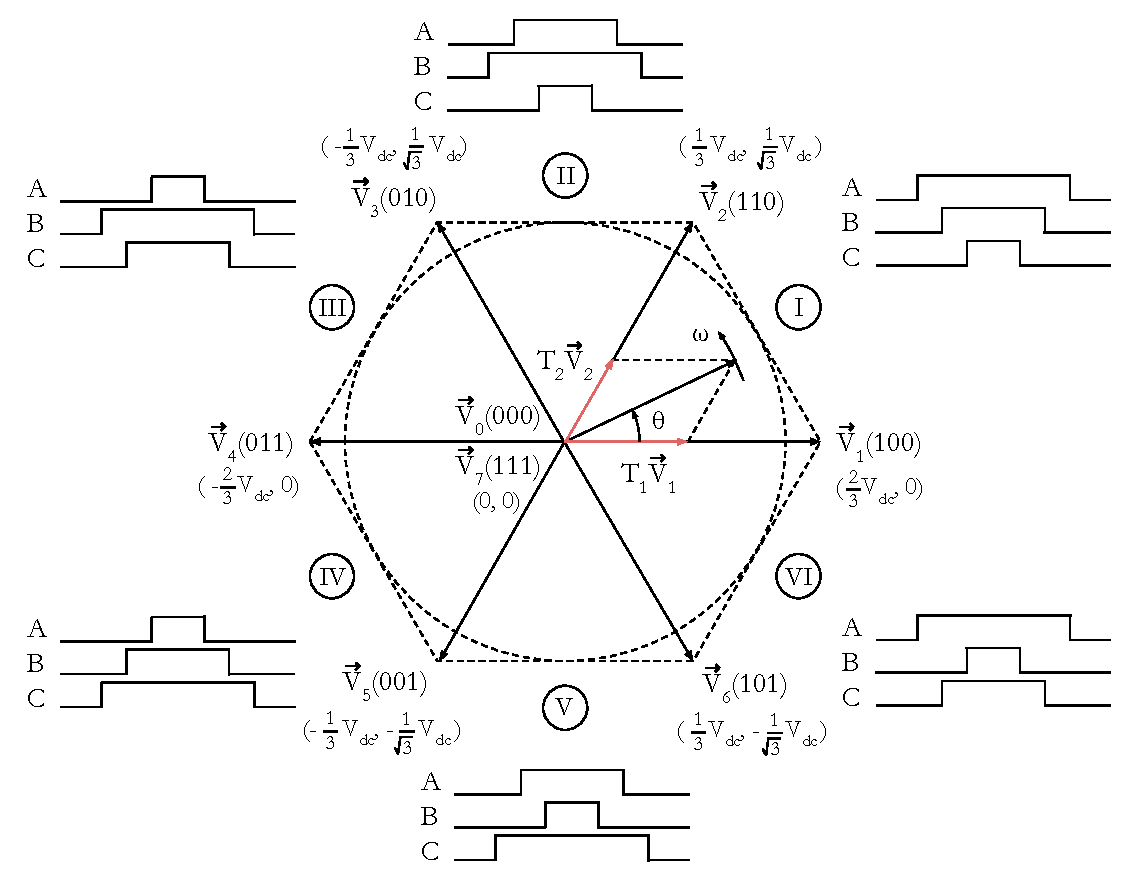
\includegraphics[width=15cm]
                { img/3_control_motor/SVPWM.pdf }
            \caption[Síntesi del vector espacial]
                { Síntesi del vector espacial. \textit{Elaboració pròpia.} }
                \label{hexagon}
        \end{figure}

        Si representem el vector de voltatge de referència en aquest marc,
        podem veure que cau entre dos estats de conmutació. Per tant, podem
        sintetitzar-lo com la suma dels vectors escalats de les commutacions
        més properes, més una contribució del vector nul 0 o 7. L'escalat dels
        vectors és directament proporcional al temps en què l'inversor es troba
        en aquell estat amb respecte el periode de commutació escollit.

        L'algorisme de SVPWM implementat es basa en la identificació del sector
        per calcular el cicles de treball que s'han de comparar amb el senyal
        triangular. El sector s'identifica inspeccionant que les components del
        vector de referència es trobin per damunt o per baix de les tres rectes
        que formen els vectors dels estats de commutació: $v_b - \sqrt{3} > 0$,
        $v_b < 0$ i $v_b + \sqrt{3} > 0$. Això genera una codificació en binari
        corresponent als nombres entre el 1 i el 6, que s'han de mapejar als
        sectors I-VI: $2 \rightarrow I,\ 6 \rightarrow II,\ 4 \rightarrow III,\
        5 \rightarrow IV,\ 1 \rightarrow V\ i\ 3 \rightarrow VI$.

        A continuació, es calculen els cicles de treball pel generador de PWM.
        Aïllant el primer dels sectors (I) en la figura \ref{hexagon}, es pot
        treure geomètricament una relació entre el vector de referència i el
        temps d'encesa de cada estat:

        \begin{equation}
            t_1 = \frac{T_s}{V_{dc}} (\frac{3}{2} V_\alpha-\frac{\sqrt{3}}{2} V_\beta);\ \ \ \ \ 
            t_2 = \sqrt{3} \frac{T_s}{V_{dc}} V_\beta;\ \ \ \ \ 
            t_0 = T_s - t_1 - t_2
        \end{equation}

        Aquest càlcul es pot aplicar de manera simètrica per la resta dels
        sectors, tenint en compte la seva posició amb respecte els eixos del
        sistema de referència $\alpha\-\beta$. Definint les variables X, Y i Z,
        i identificant el sector on ens trobem, podem calcular de manera global
        els temps $t_1$, $t_2$ i $t_0$. Si, a més, considerem que en el sectors
        impars els temps $t_1$ i $t_2$ estan intercanviats respecte els vectors
        pars, es defineixen uns temps $t_1'$ i $t_2'$ en funció de X, Y i Z,
        que es recullen en la taula de sota.

        \begin{equation}
            X = \frac{\sqrt{3}}{2}\frac{\sqrt{3}}{V_{DC}}v_\alpha;\ \ \ \ \ \
            Y = \frac{1}{2}\frac{\sqrt{3}}{V_{DC}}v_\beta;\ \ \ \ \ \
            Z = \frac{\sqrt{3}}{V_{DC}}v_\beta
        \end{equation}

        \begin{table}[!htb]
            \caption{Càlcul dels temps d'encesa}
            \centering
            
            \begin{tabular}{c r r r r r r}
                \toprule
                    {Sector} & I & II & III & IV & V & VI \\
                \midrule
                    $t_1'$ & Z & Y & X & -Z & -Y & -X \\
                    $t_1'$ & X & -Z & -Y & -X & Z & Y \\ 
                \bottomrule
            \end{tabular}
        \end{table}

        Finalment, per obtenir un temps d'encesa per cada fase agrupem els
        temps $t_1'$, $t_2'$ i $t_0$ segons el diagrama de la figura
        \ref{encesa}. La seqüència de commutació comença amb $t_0$, continua
        amb $t_1'$, segueix amb $t_2'$ i just abans d'arribar a mig periode,
        torna a $t_0$. Com que el senyal triangular és centrat, el PWM també ho
        és i per simetria la seqüència es repiteix en sentit contrari fins
        sumar un periode de commutació. Com que hi han dues aparacions de $t_1'$
        i de $t_2'$, el seu valor es divideix per la meitat; mentres que $t_0$
        es divideix entre quatre en aparèixer quatre vegades, de tal manera que
        se segueix complint $t_1' + t_2' + t_0 = T_s$. Així, els valors de
        l'amplada de cada pols, $t_x$, $t_y$ i $t_z$, es calculen com:

        \begin{equation}
            t_x = \frac{1}{4}(1-t_1'-t_2');\ \ \ \ \ \
            t_y = \frac{1}{4}(1-t_1'+t_2');\ \ \ \ \ \
            t_z = \frac{1}{4}(1+t_1'+t_2')
        \end{equation}

        Per últim, cal assignar el valor de $t_x$, $t_y$ i $t_z$ a cada una de
        les fases del commutador, seguint el esquema de la taula següent:

        \begin{table}[!htb]
            \caption{Assignació dels temps calculats a cada fase de l'inversor}
            \centering
            
            \begin{tabular}{c r r r r r r}
                \toprule
                    {Fase} & I & II & III & IV & V & VI \\
                \midrule
                    A & $t_x$ & $t_y$ & $t_z$ & $t_z$ & $t_y$ & $t_x$ \\
                    B & $t_y$ & $t_x$ & $t_x$ & $t_y$ & $t_x$ & $t_x$ \\ 
                    C & $t_z$ & $t_z$ & $t_y$ & $t_x$ & $t_x$ & $t_y$ \\ 
                \bottomrule
            \end{tabular}
        \end{table}

        \begin{figure}[!htb]
            \centering
            \captionsetup{justification=centering}
            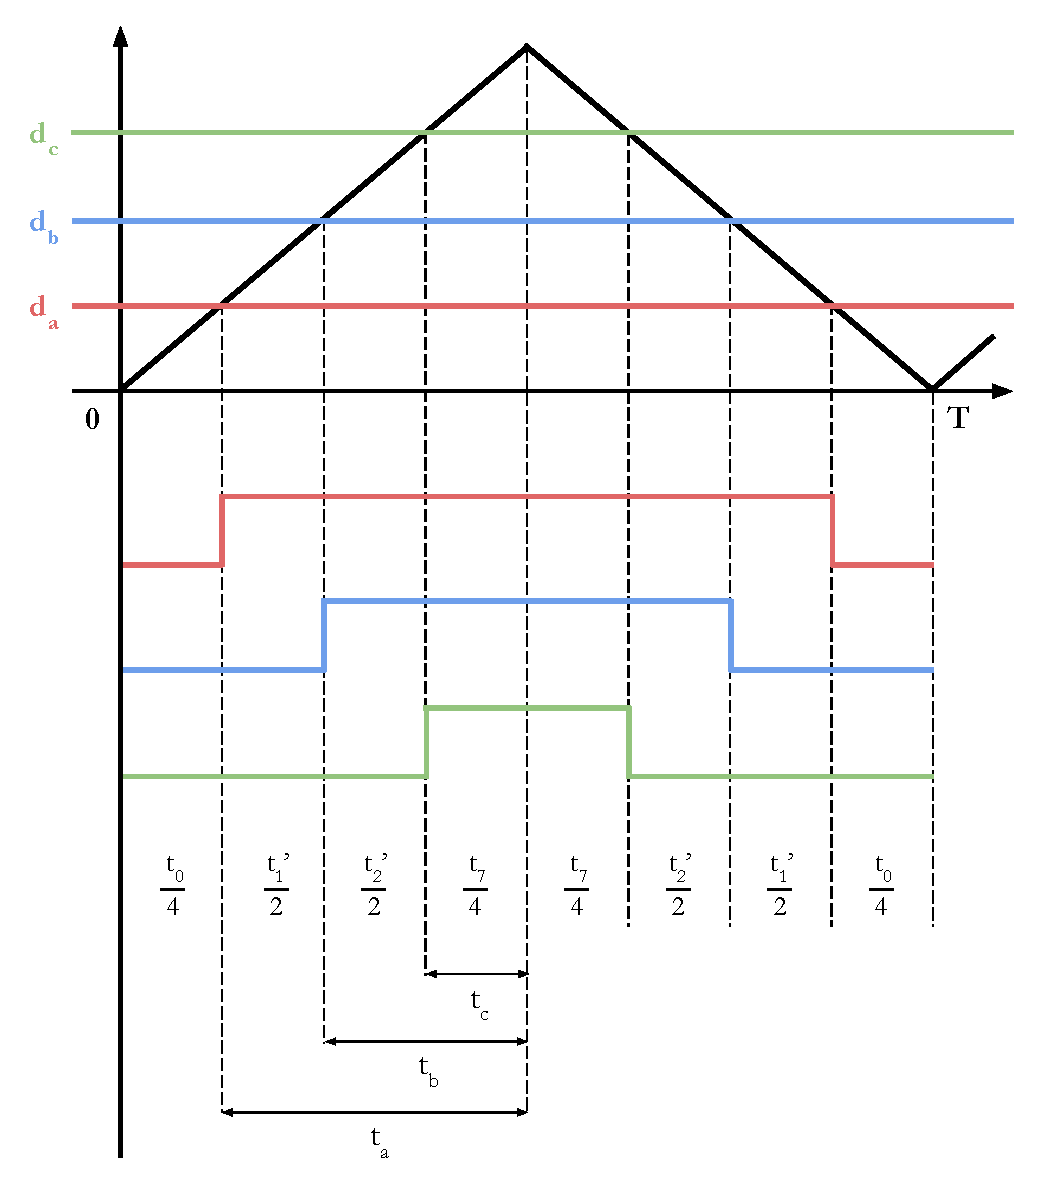
\includegraphics[width=9.5cm]
                { ../img/3_control_motor/encesa.pdf }
            \caption{ Càlcul del temps d'encesa }
            \label{encesa}   
        \end{figure}  

        \begin{figure}[!htb]
            \centering
            \captionsetup{justification=centering}
            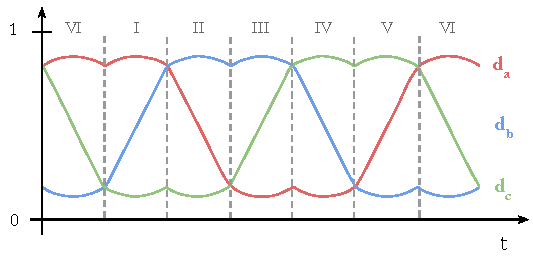
\includegraphics[width=10cm]
                { img/3_control_motor/duty.pdf }
            \caption[Cicles de treball obtinguts amb SVPWM]
                { 
                    Evolució del cicles de treball característica del SVPWM, a
                    mesura que el vector de referència passa pels diferents
                    sectors. 
                }          
        \end{figure}
    }

    \newpage
    \subsection{ Altres elements de l'algorisme de control }
    {
        L'algorisme de control necessita d'altres elements addicionals pel seu
        funcionament. 
        
        El primer d'aquests elements és la detecció de l'angle i la velocitat
        angular del rotor a partir de les mesures del resolver. Hi ha diverses
        maneres de realitzar aquesta detecció. Per aquest projecte
        s'ha decidir emprar un Resolver-to-Digital (\acs{R/D}), que es un circuit
        integrat específic per digitalitzar les mesures del resolver i que es
        basa en un sistema de control PLL. El model escollit és l'AD2S1210
        del fabricant \emph{Analog Devices} \cite{rtd}.
        
        En segon lloc hi trobem el controlador de velocitat angular. La seva
        funcionalitat principal és assegurar que la velocitat angular segueix a
        la consigna variant el valor del parell per mitjà d'una doble saturació.
    
        Per últim, s'han de considerar els elements de limitadors que
        proporcionen seguretat al control, de manera que les tensions i els
        corrents no superin els valors màxims imposats pel hardware. D'aquesta
        manera, trobem saturadors per saturar les referències de corrent $i_d*$
        i $i_q*$ i un limitador del mòdul de voltatge per saturar les
        referències de tensió $v_{d,ref}$ i $v_{q,ref}$.

        \begin{figure}[!htb]
            \centering
            \captionsetup{justification=centering, margin=1cm}
            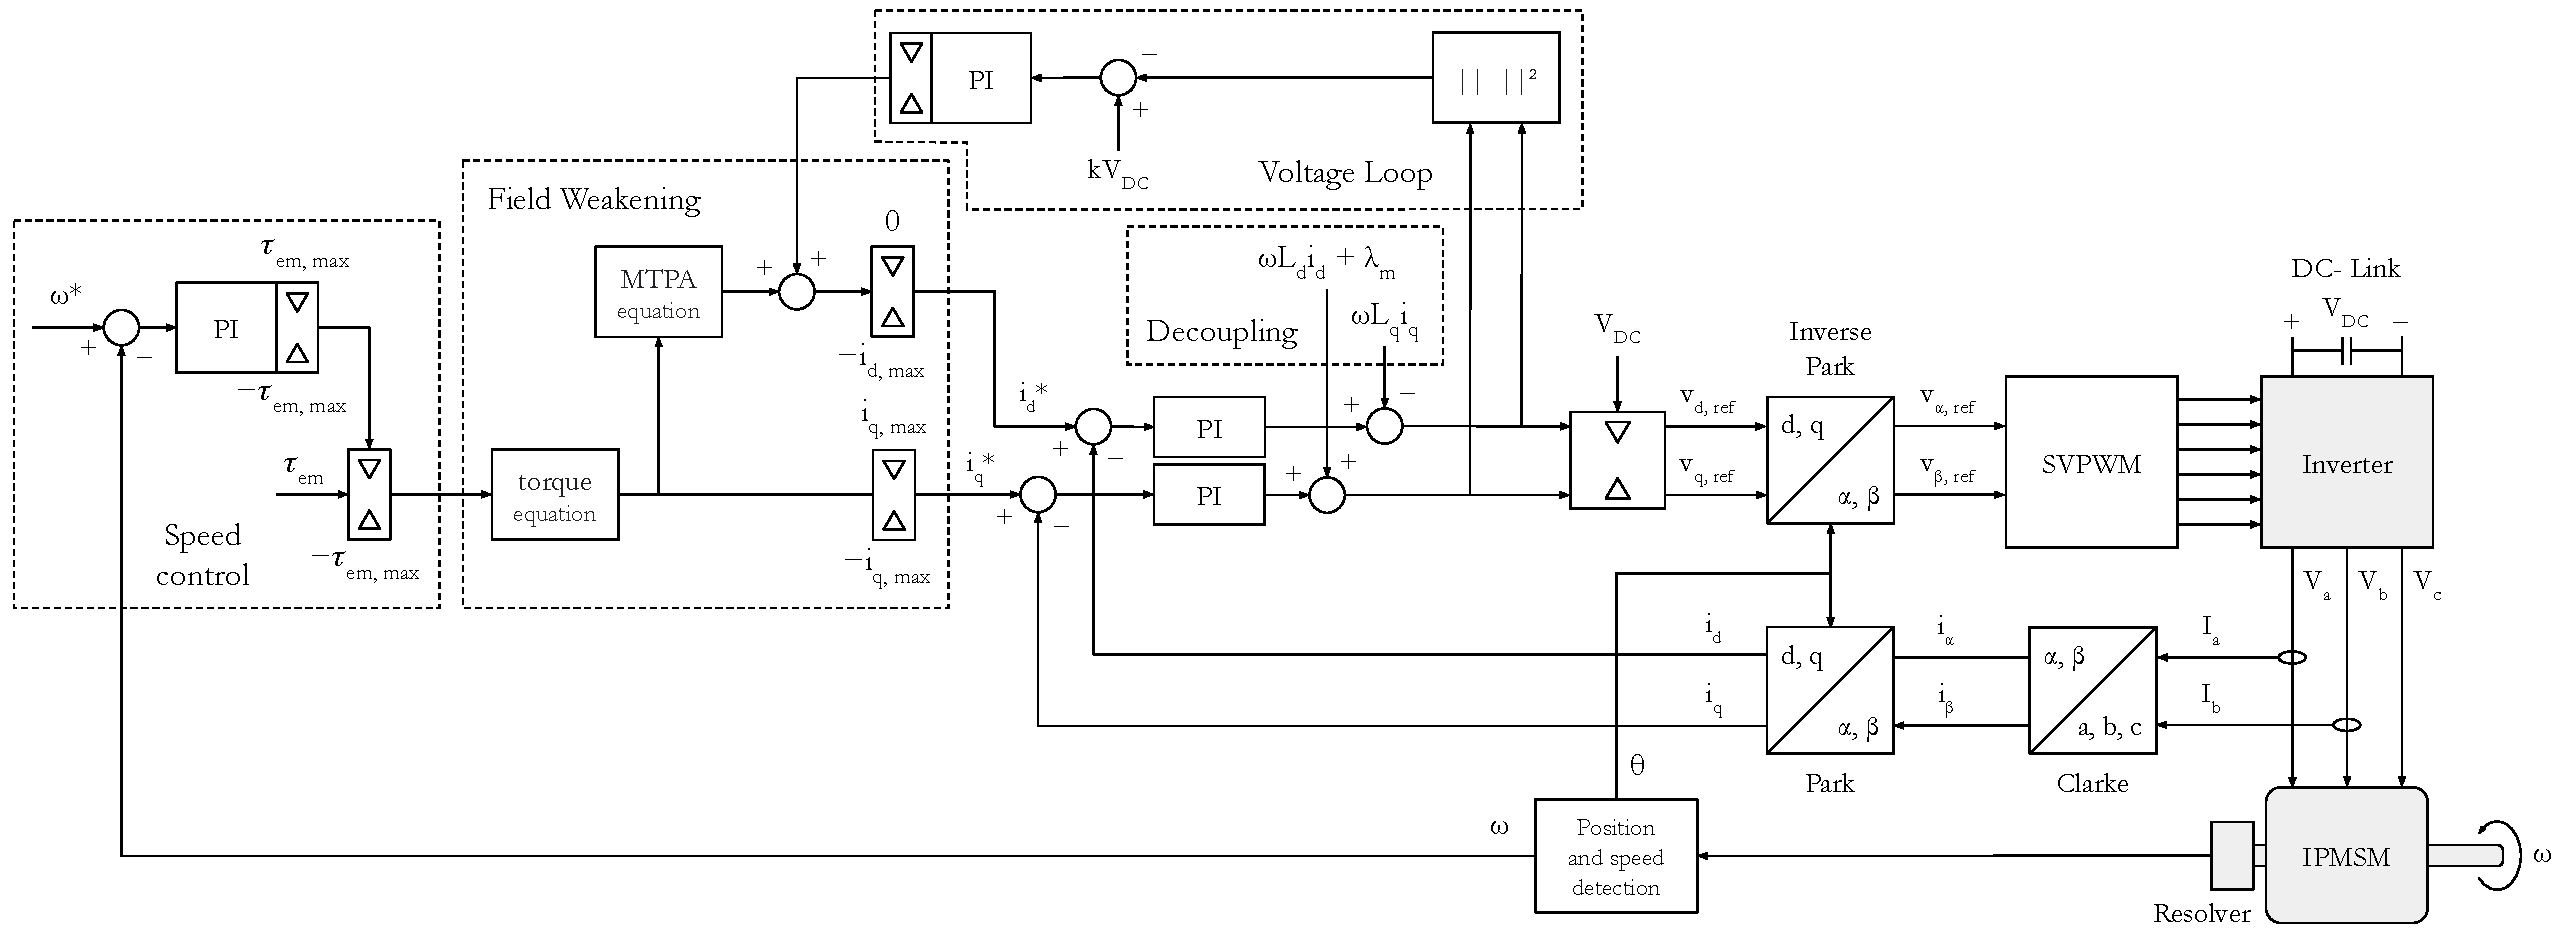
\includegraphics[width=15.75cm]
                { img/3_control_motor/control.pdf }
            \caption[Diagrama de blocs del control]
                { Diagrama de blocs complet de l'algorisme control }
            \label{diagrama}
        \end{figure}
    }
}